\documentclass[12pt]{article}
\usepackage[margin=0.7in]{geometry} 		% defines page margin
\usepackage{knitting} 				% defines \chart and \textknit
\usepackage{titling} 				% title page
\usepackage{graphicx,xspace, scrextend}	% defines space control stuff
\usepackage{tabularx, array, colortbl}	% defines tables
\usepackage{multicol} 				% defines columns
\usepackage{multirow} 				% defines multirows, combined cells in tables
\usepackage{framed} 				% defines boxes for notes and written directions
\usepackage[x11names]{xcolor} 		% extends color library
\usepackage{wrapfig}
\pdfmapfile{+knitfont.map}

% font selection
\usepackage{palatino, moresize, sectsty}
\allsectionsfont{\sffamily}

\renewcommand{\arraystretch}{1.5} % compresses tables for pattern keys

\newcolumntype{L}[1]{>{\leftalign\arraybackslash}p{#1}}
\newcolumntype{C}[1]{>{\centering\arraybackslash}p{#1}}

% length parameters
\setlength{\parindent}{0pt} % disables indentation for paragraphs
\setlength{\columnsep}{0.7cm} % column separation in multicol environment

% color parameters
\colorlet{framecolor}{black}
\colorlet{shadecolor}{LemonChiffon1}
\colorlet{highlight}{yellow}

% custom commands
\newcommand{\comment}[1]{} % allows for multiline comments that LaTeX will ignore

\newcommand{\vocab}[1]{\emph{\textbf{#1}}} % format for highlighting definitions of stitches, vocabulary terms
\newcommand{\rowDir}[1]{\textbf{#1:}} % indent for written instructions within paragraphs

\renewcommand{\repeat}[1]{\textbf{*[#1]*}} % format for written repeats, bold with *[ stitches ]*
\newcommand{\x}{$\times$}			% times symbol but shorthand
\newcommand{\setrepeat}[2]{\textbf{[#1]}\x{#2}}		% format for repeats with set number of repetitions, bold with [ stitches ]

\newcommand{\blank}{\underline{\hspace{2em}} } % written instructions, fill-in-the-blank box
\newcommand{\highlighted}[1]{\colorbox{highlight}{#1}} % written instructions, highlight particular text


% stitch count commands
\newcommand{\increase}[1]{(\emph{+#1 
	\ifnum#1=1{st}\else{sts}\fi})}
\newcommand{\decrease}[1]{(\emph{$-$#1
	\ifnum#1=1{st}\else{sts}\fi})}
\newcommand{\stitchcount}[1]{(\emph{#1 sts})}

% marker instructions
\renewcommand{\pm}[1]{\emph{pm #1}} % place stitch marker
\newcommand{\sm}{\emph{sm}} % slip marker
\renewcommand{\rm}[1]{\emph{rm #1}} % remove stitch marker

% thick horizontal line
\makeatletter \newcommand{\thickhline}{
    \noalign {\ifnum 0=`}\fi \hrule height 1.5pt
    \futurelet \reserved@a \@xhline
}
\makeatother

% custom environments
\newenvironment{frnote}
    {% framed environment for pattern notes
    	\setlength{\FrameRule}{1.5pt}
    	\def\FrameCommand{\fboxrule=\FrameRule\fboxsep=\FrameSep \fcolorbox{framecolor}{shadecolor}}
    	\MakeFramed {\FrameRestore}}
    {\setlength{\FrameRule}{1pt}
	\endMakeFramed}

\newenvironment{frdirection}
    {% framed environment for written directions
	\def\FrameCommand{\fboxrule=\FrameRule\fboxsep=\FrameSep \fbox}
   	\MakeFramed {\advance\hsize-\width \FrameRestore}
    	\addmargin[1.5cm]{0pt}}
    {\endaddmargin
	\endMakeFramed}

\newenvironment{unframed}
    {% unframed environment for written directions
	\begin{addmargin}[2em]{0pt}
	\setlength{\parindent}{-2em}}
    {%\vspace{1em}
	\setlength{\parindent}{0em}
	\end{addmargin}}

\title{There and Back Again (TABA)} % pattern name here
\author{Shanel Wu (Piper Nell)}

\begin{document}

%%%%%%%%%%%%%%%%%%%%%%%%%%%%%%%%%%%%%%%%%%%%%%%%%%
% TITLE PAGE 
\begin{titlingpage}

% COVER PHOTO
% uncommend line below if you want a background fill image
% \ThisLRCornerWallPaper{1.0}{image.jpg} 

{\fontfamily{qag}\selectfont
\HUGE\textbf{\thetitle}\\ % adjust this space
\normalsize\theauthor
}

\begin{multicols}{2}

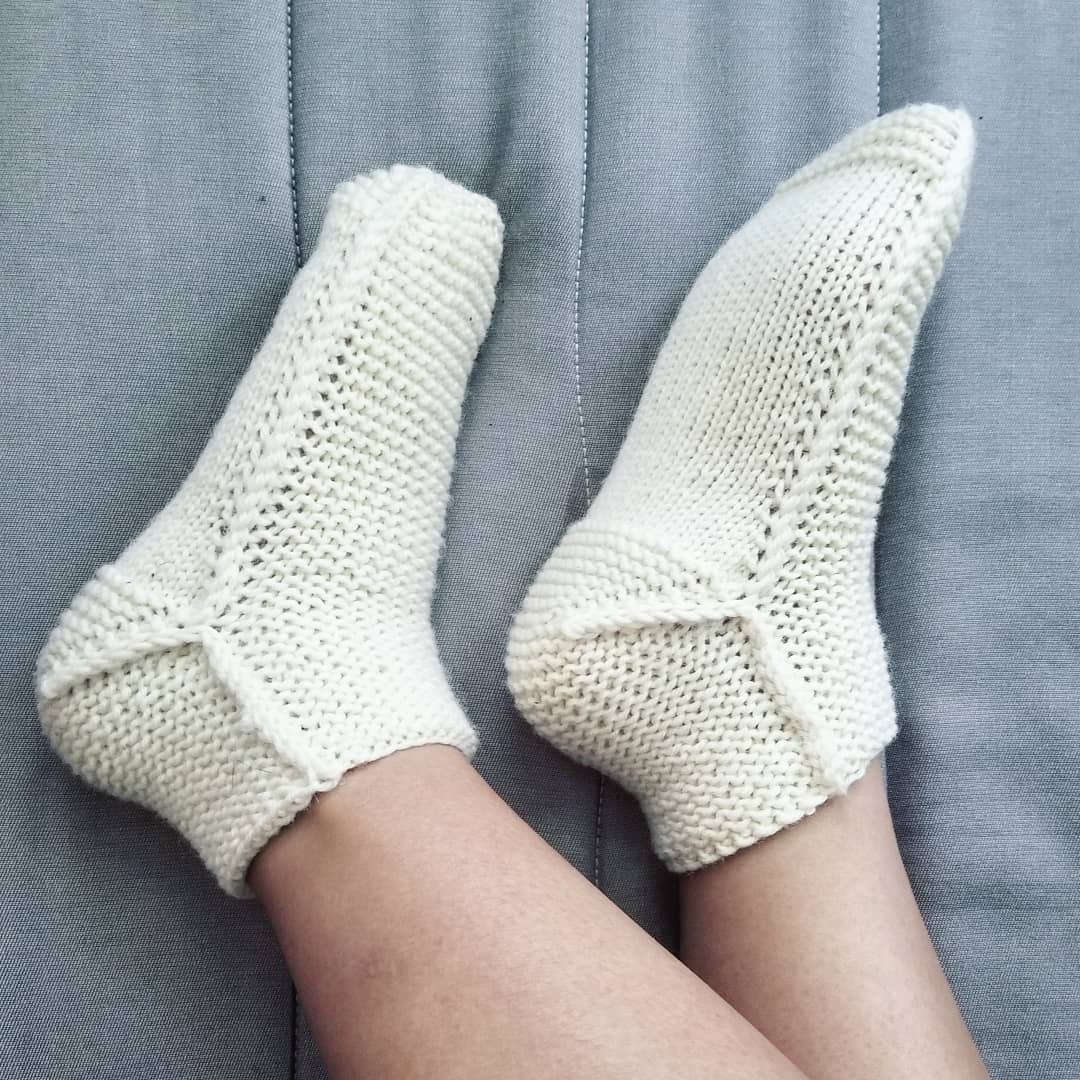
\includegraphics[width=\linewidth]{taba.jpg}

% Cute description here
\small
\vspace{-1em}
\subsection*{Sizing: XS (S, M, L)}

Fits baby (child/adult narrow, adult medium, adult wide) feet. Sizes correspond to foot widths of 2 (3, 4, 5)" or 5 (7.5, 10, 12.5) cm. Each size defaults to a foot length of 4 (7, 9, 11)" or 12.5 (17.5, 22.5, 27.5) cm, but can be adjusted by following the instructions on the following page. Select size based on foot width.

\subsection*{Yarn Requirements}

% yardage, number of colors, etc.
40 (85, 140, 200) yds of wool or wool-blend worsted weight yarn. One 100g skein will make most sizes.

% also include: sample yarn, other yarn suggestions
\emph{Sample: Diamond Pure Wool SW in ``Corn Silk"}

\subsection*{Gauge: 5 sts/1" (flexible row gauge)}

% sample measurements, gauge, notes on ease, etc.
Gauge is measured over slightly stretched stockinette stitch. A dense fabric is necessary for long-wearing socks. If you obtain a gauge tighter than 5 sts/1", work a wider sock instead of switching needle sizes.

\vfill
\columnbreak
\subsection*{Tools}

\begin{itemize}
\item US4/3.5mm (or size needed to obtain tight gauge) in any style % NEEDLES
\item tapestry needle
\item 1 removable stitch marker% STITCH MARKERS
\end{itemize}

\subsection*{Techniques}

This pattern is suitable for an advanced beginner. % DIFFICULTY LEVEL
Prior to knitting this pattern, you should be familiar with casting on, knitting, purling, k2tog, kfb, and slipping stitches. % PREREQUISITE TECHNIQUES
For a complete list of stitches used, see Pattern Key.

% discuss any special techniques and tutorials included

\subsection*{Pattern Key}

% abbreviation key - fill in with all abbreviations/stitch patterns used in design: written abbreviation, full stitch name or explanation
% try to keep them in sequential order as they appear in the pattern, or in an order that builds upon previous definitions
% chart symbols included in separate keys attached to their respective charts
% stitches with explanations must first be BOLDED, followed by colon then explanation
\begin{center}
{\renewcommand{\arraystretch}{1.5}
\begin{tabular}{| C{0.2\linewidth}  p{0.6\linewidth} | }
\thickhline \rowcolor{shadecolor} 
\textbf{Written}	& \textbf{Description} \\ \thickhline
CO 	& cast on \\
BO 	& bind off \\
RS 	& right side \\
WS 	& wrong side \\
k	&  knit \\
p	& purl   \\
k2tog 	& knit 2 together \\
sl 	& slip st (stitch) purlwise \\ 
sl1 wyib & sl 1 st with yarn in back \\
sl1 wyif & sl 1 st with yarn in front \\
psso 	& pass slipped st over \\
kfb 	& knit front back \\
\hline
\end{tabular}
}
\end{center}

~\\
\vfill
\end{multicols}
\end{titlingpage}

%%%%%%%%%%%%%%%%%%%%%%%%%%%%%%%%%%%%%%%%%%%%%%%%%%
% FOREWORD

\section*{Construction}
\small \begin{multicols}{2}
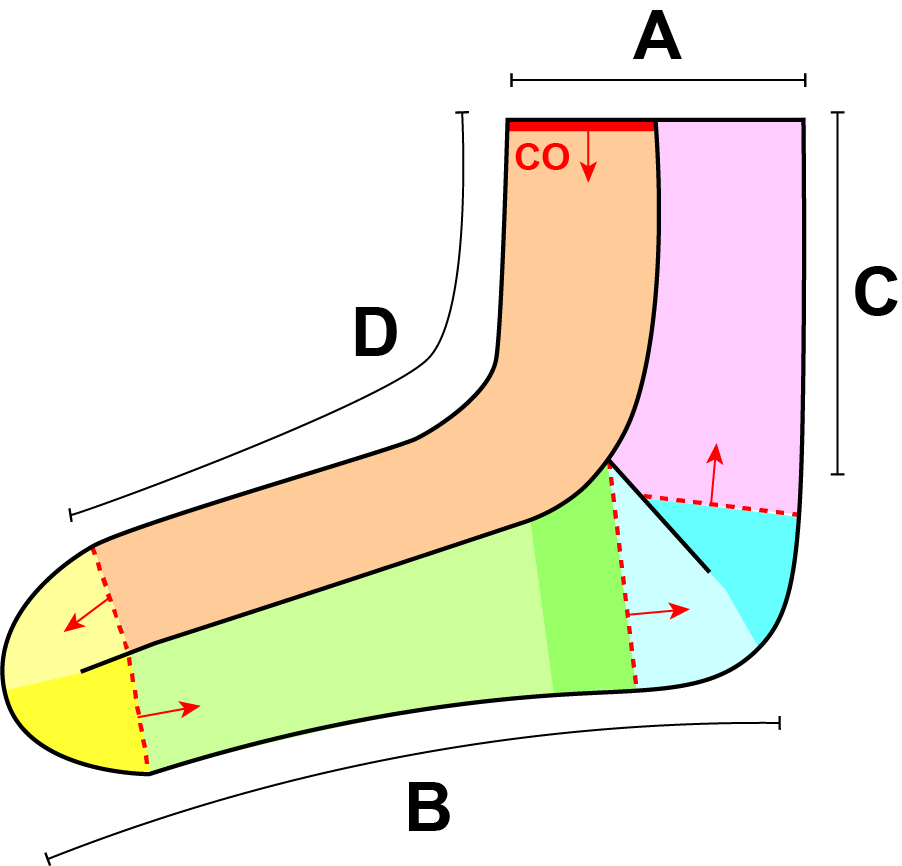
\includegraphics[width=.9\linewidth]{TABAschematic.png}
\columnbreak 
\begin{addmargin}[-2em]{0em}
{\normalsize\textbf{\textsf{A: Foot Width}}} \hspace{.5em} 2 (3, 4, 5)" / 5 (7.5, 10, 12.5) cm \\

{\normalsize\textbf{\textsf{B: Foot Length}}} \hspace{.5em} 4 (7, 9, 11)" / 10 (17.5, 22.5, 27.5) cm \\

{\normalsize\textbf{\textsf{C: Leg Height}}} \hspace{.5em} 1 (2, 3, 3)" / 2.5 (2.5, 5, 5) cm \\

{\normalsize\textbf{\textsf{D: Front Length}}} 5 (8, 11, 13)"  / 12.5 (20, 27.5, 32.5) cm \\

\emph{Leg height and front length given for short cuff option.}

The sock begins with the front cuff, proceeds down the foot, bends around the toe to complete the sole and heel, then returns to the back cuff. Each colored section in the schematic corresponds to a numbered section in the instructions.
\end{addmargin}
\end{multicols}

\subsection*{Adjusting Length/Height}

\begin{tabular}{p{0.2\linewidth} p{0.8\linewidth}}
\textbf{Foot Length: \blank} &  Measure your foot from heel to toe to determine the foot length of your socks. \\

\textbf{Leg Height: \blank} & For a \emph{short} sock as shown in the sample, divide the foot length by 3 or by 4, depending on preference. For a long sock, divide the foot length by 2. \\

\textbf{Front Length: \blank} & Add the foot length and the leg height. For all sizes \emph{except the XS}, subtract 1". 
\end{tabular}

\subsection*{Adjusting Width}
Adjusting width will be a more extensive modification. If none of the written sizes suits your needs (maybe you're modifying for a different gauge or more/less ease), you can CO any number of stitches to obtain your desired width. At the toe, work \textbf{Row 2} an even number of times until you decrease to approximately a third of your CO sts. At the gusset increases, repeat \textbf{Rows 9 and 10} until you've increased by a third of the CO stitch count. Work the heel decreases until you decrease to a third of the initial heel stitch count. Increase back to the CO stitch count to complete the sock.

\vspace{-1em}
\begin{tabular}{p{0.2\linewidth} p{0.8\linewidth}}
\begin{flushleft}\emph{\textbf{Approximate Yardge Required:} Modifying the measurements will affect the yarn required. Assuming that you are using the written gauge, this table estimates the amount of yarn you will need for certain sizes.} \end{flushleft}
&
\begin{center}
\begin{tabular}{| C{0.15\linewidth} | C{0.15\linewidth}  C{0.15\linewidth}  C{0.15\linewidth}  C{0.15\linewidth} |}
\thickhline
~ 	& \multicolumn{4}{c |}{width} 	\\
foot length	& 2" 		& 3" 		& 4" 		& 5" 	\\ \thickhline
4"	& \highlighted{40}		& 60		& 		& 	\\
7"	& 55		& \highlighted{85}		& 110		& 	\\
9"	& 		& 105		& \highlighted{140}		& 175	\\
10"	& 		& 120		& 155		& \highlighted{200}	\\
11"	& 		& 		& 170		& 220	\\
12"	& 		& 		& 185		& 235	\\ 
\hline
\end{tabular}\end{center}\end{tabular}

\normalsize
\newpage
%%%%%%%%%%%%%%%%%%%%%%%%%%%%%%%%%%%%%%%%%%%%%%%%%%
% BEGIN INSTRUCTIONS

\section*{1. Front and Instep}

CO 10 (15, 20, 25) sts 
using the long tail cast on. Place a removable stitch marker in the last CO st (i.e. the first st you will work) to mark the beginning of a RS row.

\rowDir{Row 1} sl1 wyif, k to end.

Repeat Row 1 on both the RS and WS (garter stitch)
until work measures 5 (8, 11, 13)" or 12.5 (20, 27.5, 32.5) cm from CO, 
ending after a WS row. 

\begin{wrapfigure}{R}{0.25\linewidth}
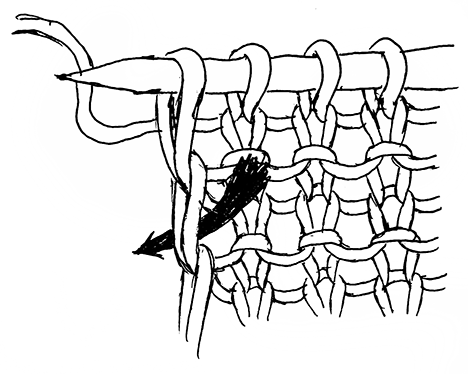
\includegraphics[width=\linewidth]{punk.png}
\emph{\small \textbf{A:} Insert R needle in this direction to pick up and knit in selvedge.}

\vspace{4em}
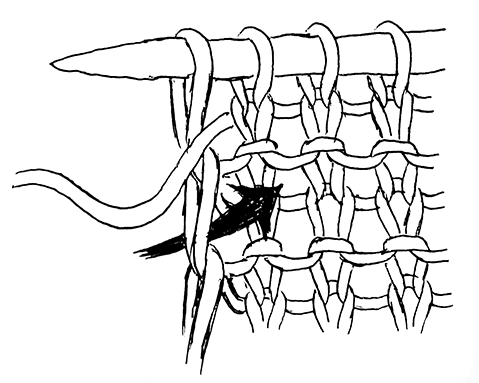
\includegraphics[width=\linewidth]{punp.png}
\emph{\small \textbf{B:} Insert R needle in this direction to pick up and purl in selvedge.}
\vspace{-6em}
\end{wrapfigure} \leavevmode

\section*{2. Toe}

\subsection*{Part A}
Work Row 2 a total of 6 (10, 14, 18) times 
until 4 (5, 6, 7) sts remain.

\rowDir{Row 2 (Decrease Row)} sl1 wyif, k to 3 sts from end, k2tog, k1. \\\decrease{1}

\subsection*{Part B}

Work Rows 3 and 4 once to set up the second half of the toe.

\rowDir{Row 3 (RS)} sl1 wyif, k to 2 sts from end, kfb, sl1 wyib, pick up and knit 1 st in the first selvedge st below (see diagram \vocab{A}), psso and turn. \increase{1}

\rowDir{Row 4 (WS)} sl1 wyif, k to 2 sts from end, kfb, sl1 wyif, pick up and purl 1 st in the first selvedge st below (see diagram \vocab{B}), psso and turn. \increase{1}

~\\
Then, repeat Rows 5 and 6 a total of 2 (4, 6, 8) times 
until you return to 10 (15, 20, 25) sts.

\rowDir{Row 5 (RS Increase Row)} sl1 wyib, k to 2 sts from end, kfb, sl1 wyib, pick up and knit 1 st in selvedge, psso and turn. \increase{1}

\rowDir{Row 6 (WS Increase Row)} sl1 wyif, k to 2 sts from end, kfb, sl1 wyif, pick up and purl 1 st in selvedge, psso and turn. \increase{1}

\section*{3. Sole}

Repeat Rows 7 and 8 (stockinette stitch) until your work measures 2.5 (4, 6, 8.5)" or 6.25 (10, 15, 21.25) cm
from the toe. Alternatively, end when your work is 1.5 (2.5, 2.5, 2.5)" or 3.75 (6.25, 6.25, 6.25) cm from the heel.

\rowDir{Row 7 (RS Joining Row)} sl1 wyib, k to 1 st from end, sl1 wyib, pick up and knit 1 st in selvedge, psso and turn.

\rowDir{Row 8 (WS Joining Row)} sl1 wyif, p to 1 st from end, sl1 wyif, pick up and purl 1 st in selvedge, psso and turn.

\pagebreak
\subsection*{Gusset Increases} 

Repeat Rows 9 and 10 a total of 2 (4, 4, 6) times
to increase for a gusset. You should end with 14 (23, 28, 37) sts.

\rowDir{Row 9 (RS)} sl1 wyib, k to 2 sts from end, kfb, sl1 wyib, pick up and knit 1 st in selvedge, psso and turn. \increase{1}

\rowDir{Row 10 (WS)} sl1 wyif, p to 2 sts from end, kfb, sl1 wyif, pick up and purl 1 st in selvedge, psso and turn. \increase{1}

\section*{4. Heel}

The heel is nearly identical to the toe, only worked over more stitches.

\subsection*{Part A}

Work Row 11 once to set up the heel.

\rowDir{Row 11 (RS)} sl1 wyib, k to 3 sts from end, k2tog, k1. \decrease{1}

Then, work Row 12 a total of 8 (14, 18, 22) times on both the RS and WS, ending after a WS row. You should end with 6 (7, 10, 13) sts.

\rowDir{Row 12} sl1 wyif, k to 3 sts from end, k2tog, k1. \decrease{1}

\subsection*{Part B}

Work Rows 13 and 14 once to set up the second half of the heel.

\rowDir{Row 13 (RS)} sl1 wyif, k to 2 sts from end, kfb, sl1 wyib, pick up and knit 1 st in the first selvedge st below (see diagram), psso and turn. \increase{1}

\rowDir{Row 14 (WS)} sl1 wyif, k to 2 sts from end, kfb, sl1 wyif, pick up and purl 1 st in the first selvedge st below (see diagram), psso and turn. \increase{1}

~\\
Then, repeat Rows 15 and 16 a total of 1 (3, 4, 5) times until you return to 10 (15, 20, 25) sts.

\rowDir{Row 15 (RS Increase Row)} sl1 wyib, k to 2 sts from end, kfb, sl1 wyib, pick up and knit 1 st in selvedge, psso and turn. \increase{1}

\rowDir{Row 16 (WS Increase Row)} sl1 wyif, k to 2 sts from end, kfb, sl1 wyif, pick up and purl 1 st in selvedge, psso and turn. \increase{1}

\begin{wrapfigure}{R}{0.45\linewidth}
\vspace{-2em}
\begin{frnote} \ssmall
Pattern \copyright 2018 Shanel Wu. All rights reserved. In purchasing this pattern, you agree to print and use this pattern only for personal use. Do not redistribute or sell paper or electronic copies of this pattern.
\end{frnote}
\vspace{-5em}
\end{wrapfigure} \leavevmode

\section*{5. Back}

Repeat Rows 17 and 18 until the last selvedge st has been worked, ending after a RS row.



\rowDir{Row 17 (RS Joining Row)} sl1 wyib, k to 1 st from end, sl1 wyib, pick up and knit 1 st in selvedge, psso and turn.

\rowDir{Row 18 (WS Joining Row)} sl1 wyif, k to 1 st from end, sl1 wyif, pick up and knit 1 st in selvedge, psso and turn.

On the next WS row, BO all stitches loosely for a stretchy edge. Cut yarn and weave in ends. Repeat for second sock, and then enjoy your toasty toes!



%%%%%%%%%%%%%%%%%%%%%%%%%%%%%%%%%%%%%%%%%%%%%%%%%%
% APPENDICES (IF ANY)

\end{document}